\section{Feature selection}
So far we've dealt only with the complexity of the model, but what about the features? 
We'd like to select only those features that are more relevant in order to have the right quality and quantity. The idea of starting from a full-model $\mathcal{M}_{\text{all}} = \{x_1, x_2, \ldots, x_p\}$ we want to derive a \textbf{selected-feature model} $\mathcal{M}_S = \{x_j : j \in S\}, S \subseteq \{1, \ldots, p\}$ with the \textit{the best balanca between prediction accuracy and complexity}.

\begin{figure}[h]
    \centering
    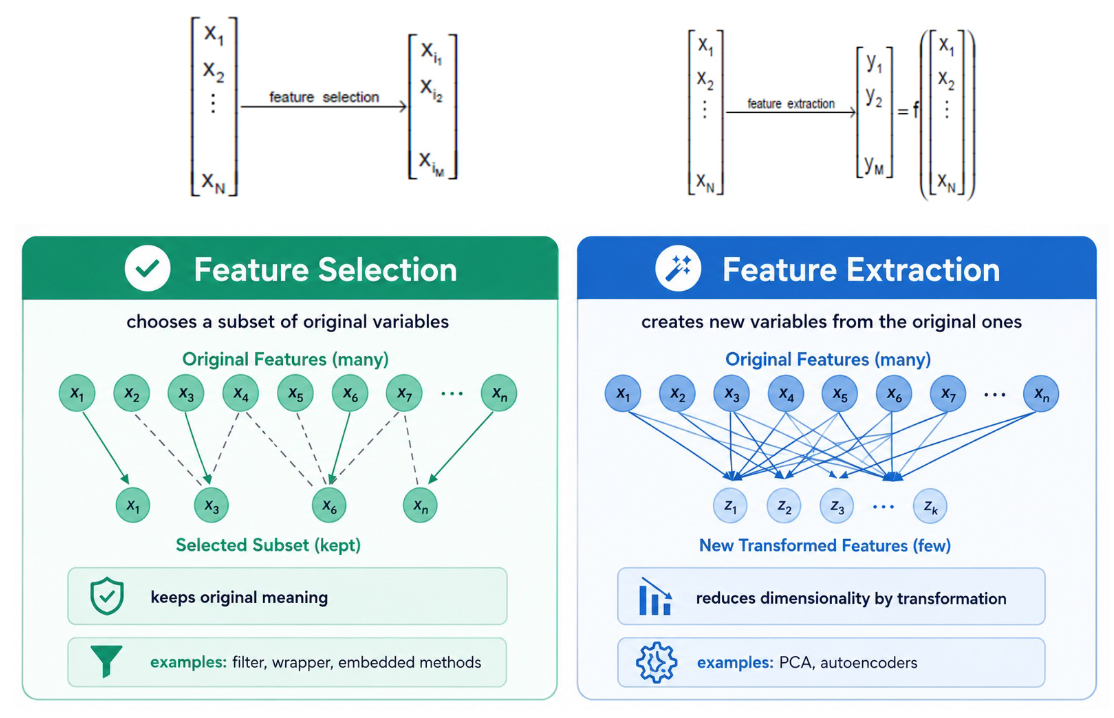
\includegraphics[width=0.7\linewidth]{img//feature_selection/feature_selection_vs_extraction.png}
    \caption*{Feature selection is different from feature extraction moethods like PCA: here we want only to select those features among those already present.}
\end{figure}

\subsection{Filter methods}
In this class of methods we rank the features following some metric that doesn't depend on the actual model and we pick only the top ones.\\
\begin{figure}[h]
    \centering
    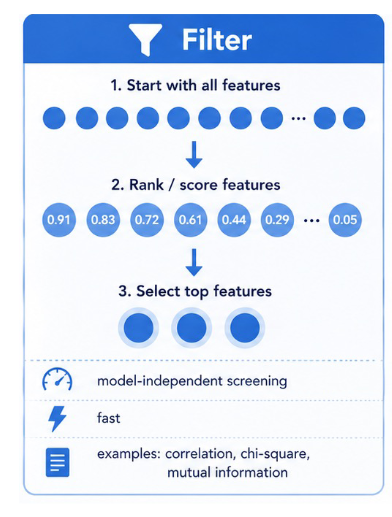
\includegraphics[width=0.3\linewidth]{img//feature_selection/filter_summary.png}
\end{figure}

Examples of scoring metrics \textcolor{gray}{(just examples, you don't need to know them)}:
\begin{itemize}
    \item correlation with the outcome;
    \item t-test / ANOVA;
    \item chi-square test for categorical features;
    \item mutual information;
    \item variance threshold;
    \item univariate logistic regression p-values.
\end{itemize}

\begin{minipage}[t]{0.45\textwidth}
  \textcolor{green!60!black}{\textbf{Pros:}}
  \begin{itemize}
    \item very simple
    \item very fast
    \item useful when $p$ is large
  \end{itemize}
\end{minipage}
\begin{minipage}[t]{0.45\textwidth}
  \textcolor{red}{\textbf{Cons:}}
  \begin{itemize}
    \item usually considers features one at a time;
    \item may miss interactions;
    \item may keep redundant variables;
    \item does not directly optimize predictive performance.
  \end{itemize}
\end{minipage}

\subsubsection{Multivariate Filering}
With this family of algorithms each feature based on the other selected: $score(x_j,Y,S)$ where $Y$ are the outcomes and $S$ are the selected features.\\
\vspace{0.2cm}
One metric used is the \textbf{minimum Redundancy Maximum Relevance (MRMR)} which selects the features balancing the relevance fo the single feture for $Y$ and the low redundancy of the features.
$$
\text{score}(x_j) = I(x_j; Y) - \frac{1}{|S|}\sum_{x_k \in S} I(x_j; x_k)
$$
where $I(x_j; Y)$ := relevance of the feature for the score, $I(x_j; x_k)$ := redundant information within features.

wrapper : select the fatures that give the best performance for my model (basically choose those features that give the best result for my model,I pick what's better for me)
embedded: do both feature selection and model selection at the same time.

\subsection{Wrapper methods}
In this class of methods we select those features giving the best result for our model, so these are \textbf{model-dependent} algorithms and are often used together with cross-validation to select the subsets.
$$
S^*=\arg\max_S\ CV(\ \text{perf}(S)\ )
$$
\begin{figure}[h!]
    \centering
    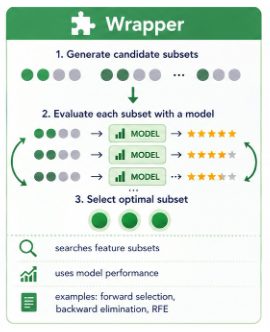
\includegraphics[width=0.3\linewidth]{img//feature_selection/wrapper_methods.png}
\end{figure}
\newpage

\begin{minipage}[t]{0.45\textwidth}
  \textcolor{green!60!black}{\textbf{Pros:}}
    \begin{itemize}
        \item directly bounded to model performance
        \item they'reable to capture fatires interactions
    \end{itemize}
\end{minipage}
\begin{minipage}[t]{0.45\textwidth}
    \textcolor{red}{\textbf{Cons:}}
    \begin{itemize}
        \item computational expensive
        \item may overfit, need careful cross-validation
    \end{itemize}
\end{minipage}
    
\subsubsection{Forward selection}
Start with no features and one at a time, verifying if by adding it the model performance improve. This type of methods is useful when only a small subset of features is relevant in a large number of predictors.
\subsubsection{Backward elimination}
Start with all the features and remove it one at a time. We choose the feature to remove based on which causes the minor loss in model performance. Useful to simplify the model when it's easy to fit.
\subsubsection{Recursive Feature Elimination (RFE)}
Start with all features, fit a model, rank features by model-based importance, remove the weakest feature or features, and repeat. Useful when the model gives some feature importance score, like the coefficients in linear regression.

\subsection{Embedded methods}
With embedded methods we embedd the feature selection directly into the learning algorithm, allowing it to determining automatically which features are more important.\\ 
The two main methods are \textbf{coefficient shrinkage} in which we try to shrink down a coefficient to zero, and \textbf{feature importance} (see later).\\
\begin{figure}[h]
    \centering
    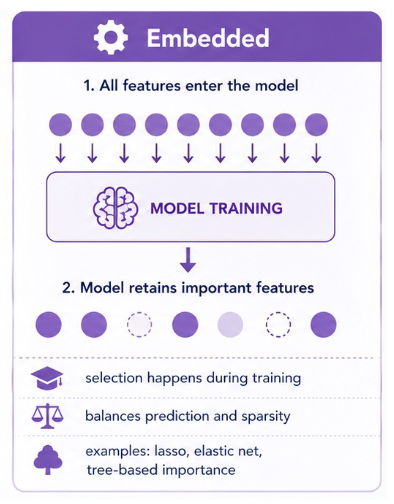
\includegraphics[width=0.3\linewidth]{img//feature_selection/embedded_methods.png}
\end{figure}
\textcolor{green!60!black}{\textbf{Pros:}}
\begin{itemize}
    \item computationally efficient since we train the model only once
    \item the are able to capture interaction betwwen the model and the features
    \item allow to reduce overfitting by focusing only on the most relevant features
\end{itemize}
\newpage
\subsection{Regularization}
If we take in consideration a std linear predictor $\eta(x)=\beta_0+\beta_1x_1...+\beta_px_p$ in general we have that the coefficients become unstable when $p$ is large. The idea of regularization is to \textbf{modify the fitting objective} in order to penalize the model complexity \arrow  we add a bias to favor the selection of simpler models.
$$
\text{Loss}(\beta) +\lambda\cdot\text{penalty}(\beta)\quad \lambda:=\text{regulatization strength}\ge 0
$$

By doing so we can't intepret easily the coefficient as in std regression, so to obtain an interpretable model we can run the regularization, select the most important/relevant features and re-fit the model only on those.

\subsubsection{Ridge regression}
As penaly we use the square of the coefficients, $L_2$. By doing so the coefficients will go toward zero (but not zero) as we set a stronger $\lambda$  and keeps in the model all the variables. It also helps with correlated predictors and reduce model variance. However it never preforms a feature selection 'cause coefficients are never drawn to zero, they only become very small, so it's not strictly an embedded feature selection method.
$$
L_2=\lambda\sum_{j=1}^p\beta_j^2
$$
\begin{figure}[h]
    \centering
    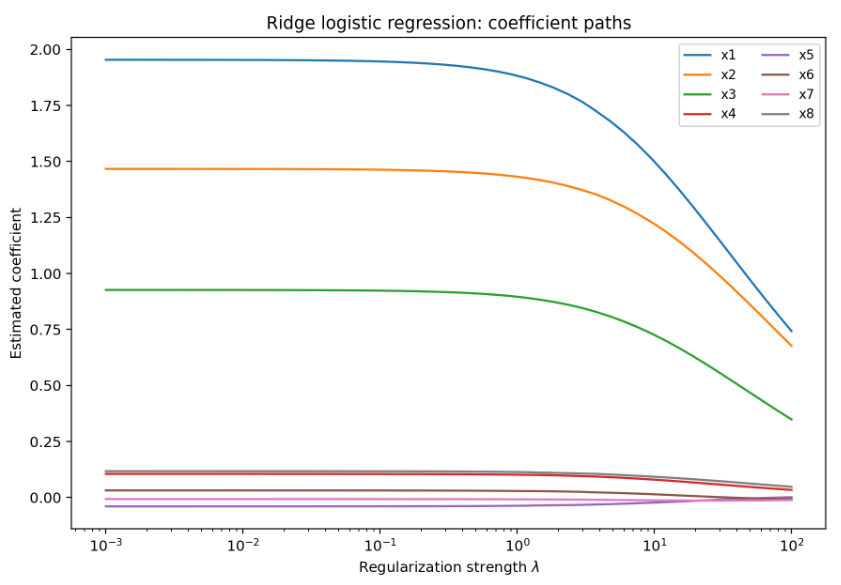
\includegraphics[width=0.4\linewidth]{img//feature_selection/ridge_regression.png}
\end{figure}

\subsubsection{Least Absolute Shrinkage and Selection Operato (LASSO) regression}
Here instead we use the $L_1$ penalty. Using this penalty function allows us to shrink coefficient down to zero, performing de facto embedded feature selection along with regularization.
$$
L_1=\sum_{j=1}^p|\beta_j|
$$
\begin{figure}[h]
    \centering
    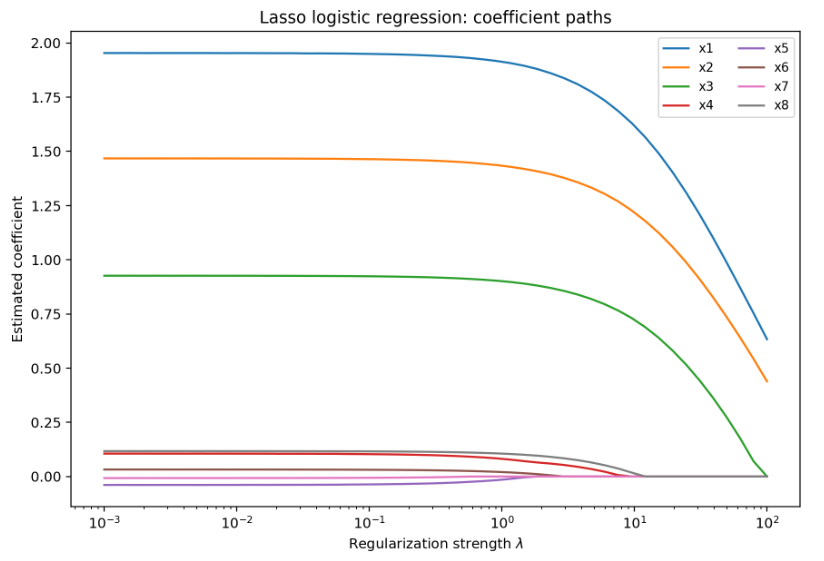
\includegraphics[width=0.4\linewidth]{img//feature_selection/lasso.png}
\end{figure}

\vspace{0.2cm}
Due the ability of shrinking coefficient up to 0 LASSO migh produce \textbf{sparse models} := models in which some original features are excluded (in other words, the coefficients are zero). The produced models are more sparse as $\lambda$ increases, so the regulatization strength controls both the shrinkage and the number of selected features.\\
\begin{figure}[h]
    \centering
    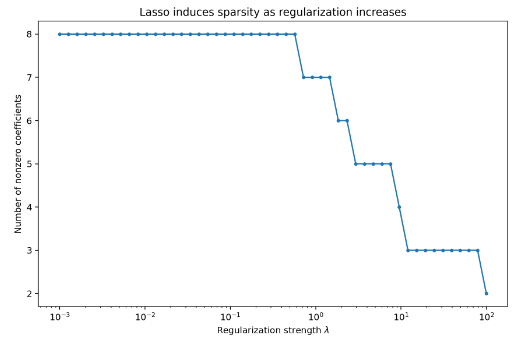
\includegraphics[width=0.4\linewidth]{img//feature_selection/lasso_sparse_model.png}
\end{figure}
However with LASSO we can't choose which coefficient are shrink to 0.\\

How do we choose the right $\lambda$? We use validation/cross-validation.
$$
\hat{\lambda}=\arg\max_\lambda\ CV_{performance}(\lambda)
$$
\begin{figure}[h]
    \centering
    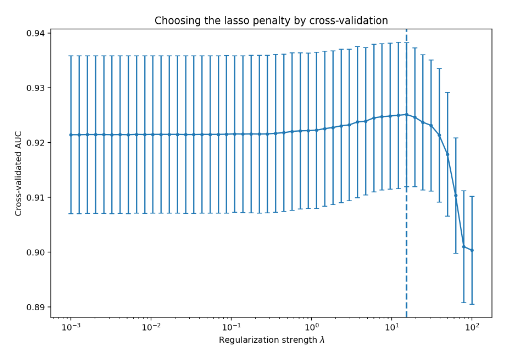
\includegraphics[width=0.4\linewidth]{img//feature_selection/reg_choosing_strength.png}
\end{figure}

What happens when there are two strongly correlated predictors?\\
\begin{description}
    \item[Ridge] tends to distribute the weight across correlated predictors
    \item[LASSO] tends to choose on predictor and shrinking it more rapidly than the other one
    \arrow this means that LASSO might be unstable when predictors are highly correlated
\end{description}
\begin{figure}[h]
    \centering
    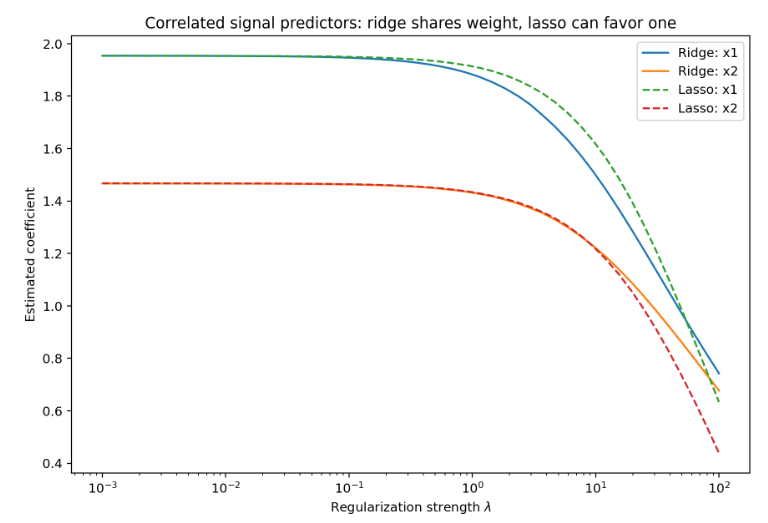
\includegraphics[width=0.4\linewidth]{img//feature_selection/lasso_stability.png}
\end{figure}
So in order to have a clearer idea we should run LASSO several times and compare the results: if some feature remain consistently revalant across all runs, then it's probably very relevant. Thereofre LASSO can be used also to exploit collinearity. 